\documentclass[10pt, a4paper]{article}
\usepackage{graphicx}
\usepackage{amsmath, amssymb, amsthm}
\usepackage{mathrsfs}
\usepackage{geometry}
\usepackage{enumitem}
\usepackage{tikz}
\usepackage{hyperref}
\usepackage{booktabs}
\usepackage{fullpage}
\usepackage{pgfplots}
\usepackage{multicol}
\usepackage[siunitx]{circuitikz}
\usepackage{caption}
\usepackage{float}
\usepackage{multirow}
\usepackage{tikz-cd}
\usepackage[utf8]{inputenc}
\usepackage{pst-eucl}
\geometry{margin=1in}

\title{Mathematica Compendium}
\author{Miguel Antonio Méndez Hernández}
\date{April 2025}

\begin{document}

\maketitle
\thispagestyle{empty}
\newpage
\tableofcontents
\newpage

\section{Propositional Logic}
Propositional logic is also called Boolean logic as 
it works on 0 and 1. In propositional logic, we use symbolic variables to represent the logic, and we can use any symbol for a representing a proposition, such \textit{A, B, C, P, Q, R}, etc. Propositions can be either \textit{true} or \textit{false}, but it cannot be both.

\subsection{Logic Operators and Truth Tables}
\smallskip
\begin{multicols}{2}

	\subsection*{NOT (\(\neg\), \(\sim\))}

	\begin{tabular}{cc}
		\toprule
		\(A\) & \(\neg A\) \\
		\midrule
		0   & 1        \\
		1   & 0        \\
		\bottomrule
	\end{tabular}

	\vspace{1em}

	\subsection*{AND (\(\land\))}

	\begin{tabular}{ccc}
		\toprule
		\(A\) & \(B\) & \(A \land B\) \\
		\midrule
		0   & 0   & 0           \\
		0   & 1   & 0           \\
		1   & 0   & 0           \\
		1   & 1   & 1           \\
		\bottomrule
	\end{tabular}

	\vspace{1em}

	\subsection*{OR (\(\lor\))}

	\begin{tabular}{ccc}
		\toprule
		\(\)A\(\) & \(B\) & \(A \lor B\) \\
		\midrule
		0   & 0   & 0          \\
		0   & 1   & 1          \\
		1   & 0   & 1          \\
		1   & 1   & 1          \\
		\bottomrule
	\end{tabular}

	\vspace{1em}

	\subsection*{IMPLIES (\(\implies\))}

	\begin{tabular}{ccc}
		\toprule
		\(A\) & \(B\) & \(A => B\) \\
		\midrule
		0   & 0   & 1        \\
		0   & 1   & 1        \\
		1   & 0   & 0        \\
		1   & 1   & 1        \\
		\bottomrule
	\end{tabular}

	\columnbreak

	\subsection*{IFF (\(\iff\))}

	\begin{tabular}{ccc}
		\toprule
		\(A\) & \(B\) & \(A <=> B\) \\
		\midrule
		0   & 0   & 1         \\
		0   & 1   & 0         \\
		1   & 0   & 0         \\
		1   & 1   & 1         \\
		\bottomrule
	\end{tabular}

	\vspace{1em}

	\subsection*{XOR (\(\oplus\))}

	\begin{tabular}{ccc}
		\toprule
		\(A\) & $B$ & $A \oplus B$ \\
		\midrule
		0   & 0   & 0            \\
		0   & 1   & 1            \\
		1   & 0   & 1            \\
		1   & 1   & 0            \\
		\bottomrule
	\end{tabular}

	\vspace{1em}

	\subsection*{NOR (\(\downarrow\))}

	\begin{tabular}{ccc}
		\toprule
		\(A\) & \(B\) & \(A \downarrow B\) \\
		\midrule
		0   & 0   & 1                \\
		0   & 1   & 0                \\
		1   & 0   & 0                \\
		1   & 1   & 0                \\
		\bottomrule
	\end{tabular}

	\vspace{1em}

	\subsection*{NAND (\(\uparrow\))}

	\begin{tabular}{ccc}
		\toprule
		\(A\) & \(B\) & \(A \uparrow B\) \\
		\midrule
		0   & 0   & 1              \\
		0   & 1   & 1              \\
		1   & 0   & 1              \\
		1   & 1   & 0              \\
		\bottomrule
	\end{tabular}

\end{multicols}
\medskip

\subsection{Tautology and Contradiction}

\textit{- Tautology}: A logical formula that is always true.

\textit{- Contradiction}: A formula that is always false.

\newpage

\subsection{Logical Equivalences}

\textbf{Commutative Laws}
\[
	p \land q \Leftrightarrow q \land p \qquad p \lor q \Leftrightarrow q \lor p
\]

\textbf{Associative Laws}
\[
	(p \land q) \land r \Leftrightarrow p \land (q \land r) \qquad (p \lor q) \lor r \Leftrightarrow p \lor (q \lor r)
\]

\textbf{Distributive Laws}
\[
	p \land (q \lor r) \Leftrightarrow (p \land q) \lor (p \land r) \qquad
	p \lor (q \land r) \Leftrightarrow (p \lor q) \land (p \lor r)
\]

\textbf{Identity Laws}
\[
	p \land \text{T} \Leftrightarrow p \qquad p \lor \text{F} \Leftrightarrow p
\]

\textbf{Negation Laws}
\[
	p \lor \sim p \Leftrightarrow \text{T} \qquad p \land \sim p \Leftrightarrow \text{F}
\]

\textbf{Double Negation Law}
\[
	\sim(\sim p) \Leftrightarrow p
\]

\textbf{Idempotent Laws}
\[
	p \land p \Leftrightarrow p \qquad p \lor p \Leftrightarrow p
\]

\textbf{Universal Bound Laws}
\[
	p \lor \text{T} \Leftrightarrow \text{T} \qquad p \land \text{F} \Leftrightarrow \text{F}
\]

\textbf{De Morgan’s Laws}
\[
	\sim (p \land q) \Leftrightarrow (\sim p) \lor (\sim q) \qquad
	\sim (p \lor q) \Leftrightarrow (\sim p) \land (\sim q)
\]

\textbf{Absorption Laws}
\[
	p \lor (p \land q) \Leftrightarrow p \qquad p \land (p \lor q) \Leftrightarrow p
\]

\textbf{Conditional Laws}
\[
	(p \Rightarrow q) \Leftrightarrow (\sim p \lor q) \qquad \sim(p \Rightarrow q) \Leftrightarrow (p \land \sim q)
\]

\textbf{Complement Law}
\[
	p \lor \neg p \Leftrightarrow \text{T} \qquad p \land \neg p \Leftrightarrow \text{F}
\]

\textbf{Biconditional}
\[
	p \Leftrightarrow q \Leftrightarrow (p \Rightarrow q) \land (q \Rightarrow p)
\]

\textbf{Transitivity}
\[
	(p \Rightarrow q) \land (q \Rightarrow r) \Rightarrow (p \Rightarrow r)
\]

\textbf{Indirect Proof (Contrapositive)}
\[
	(p \Rightarrow q) \Leftrightarrow (\neg q \Rightarrow \neg p)
\]

\textbf{Disjunctive Syllogism (Disjunctive Exclusion)}
\[
	p \nabla q \equiv (p \lor q) \land \neg p \Rightarrow q
\]
\[
	p \nabla q \equiv(p \land q) \lor \neg  (p \land q)
\]

\subsection{Truth Tables}

Truth tables are a fundamental tool in logic that systematically show the truth value
(true or false) of a compound statement for every possible combination of the truth values of 
its individual component statements.
\\\\
Essentially, they lay out all the scenarios and the resulting truth of the overall logical expression.
This helps determine if an argument is valid, if statements are logically equivalent, or the circumstances
under which a complex statement is true or false.
\\\\
\textbf{Example:}

\begin{center}
	\begin{tabular}{|c|c|c|c|c|c|c|c|}
		\hline
		\(p\) & \(q\) & \(\neg p\) & \(\neg q\) & \(\neg p \Rightarrow q\) & \((\neg p \Rightarrow q) \land \neg p\) & \(\left[(\neg p \Rightarrow q) \land \neg p\right] \Rightarrow q\) \\
		\hline
		T   & T   & F        & F        & T                      & F                                     & T                                                                \\
		T   & F   & F        & T        & T                      & F                                     & T                                                                \\
		F   & T   & T        & F        & T                      & T                                     & T                                                                \\
		F   & F   & T        & T        & F                      & F                                     & T                                                                \\
		\hline
	\end{tabular}
\end{center}

\subsubsection{Filling a truth table}
To fill a truth table for a logical expression with truth values (True or False), you follow a specific order for the input variables. This order ensures that all possible combinations of truth values for the variables are covered.

\subsubsection{General Procedure:}
\begin{enumerate}
	\item \textbf{List all possible combinations of truth values for the input variables}: If you have \(n\) variables, the number of rows in the truth table will be \(2^n\). Each variable can be either True (T) or False (F).

	\item \textbf{Order of the input variables}:
	      \begin{itemize}[label=\(-\)]
		      \item Start by filling in the truth values for the first variable. It alternates between True and False every \(2^{n-1}\) rows.
		      \item Then for the second variable, it alternates every \(2^{n-2}\) rows, and so on.
		      \item In short: the first variable alternates every other row, the second variable every two rows, the third every four rows, and so on.
	      \end{itemize}
\end{enumerate}

\textbf{Example: } 

For 3 variables, there are \(2^3 = 8\) possible combinations of truth values. The truth values are filled in the following order:

\[
	\begin{array}{|c|c|c|c|}
		\hline
		A & B & C & \text{Expression Result} \\
		\hline
		T & T & T &                          \\
		T & T & F &                          \\
		T & F & T &                          \\
		T & F & F &                          \\
		F & T & T &                          \\
		F & T & F &                          \\
		F & F & T &                          \\
		F & F & F &                          \\
		\hline
	\end{array}
\]

The pattern for filling the input truth values
\begin{itemize}[label=\(-\)]
	\item The first column (A) alternates every 4 rows: `T, T, F, F, T, T, F, F`.
	\item The second column (B) alternates every 2 rows: `T, T, F, F, T, T, F, F`.
	\item The third column (C) alternates every row: `T, F, T, F, T, F, T, F`.
\end{itemize}

This ensures that all combinations of \(A\), \(B\), and \(C\) are covered, and you can then evaluate the logical expression for each combination.

\subsubsection*{Truth Table for the Expression \( (A \land B) \lor C \)}

\[
	\begin{array}{|c|c|c|c|}
		\hline
		A & B & C & (A \land B) \lor C \\
		\hline
		T & T & T & T                  \\
		T & T & F & T                  \\
		T & F & T & T                  \\
		T & F & F & F                  \\
		F & T & T & T                  \\
		F & T & F & F                  \\
		F & F & T & T                  \\
		F & F & F & F                  \\
		\hline
	\end{array}
\]

\subsection{Disjunctive Normal Form (DNF)}

Disjunctive Normal Form (DNF) is a standard way of writing a logical expression as a disjunction
(OR) of conjunctions (ANDs). A DNF expression consists of a series of
conjunctions of literals, where each conjunction is connected by disjunctions.

To find the DNF in a truth table take the rows of the final result where there are
true statements and bind the propositions that generated it with an AND inside parenthesis.
Repeat it with each of true rows and connect all parenthesis with OR's

\textbf{Example of DNF:}

Consider the logical expression:
\[
	(A \land B) \lor (\neg A \land C) \lor (B \land \neg C)
\]
This is in DNF because it is a disjunction (OR) of conjunctions (ANDs) of literals.

\subsection{Conjunctive Normal Form (CNF)}

Conjunctive Normal Form (CNF) is a standard way of writing a logical expression as a conjunction (AND)
of disjunctions (ORs). A CNF expression consists of a series of disjunctions of
literals, where each disjunction is connected by conjunctions.

To find the CNF proceed just as the DNF but with the "false rows and instead
of ANDs inside the parenthesis use OR and connect the terms with OR. Also add a negation before each parenthesis.

\textbf{Example of CNF:}

Consider the logical expression:
\[
	\neg (A \lor B) \land \neg (\neg A \lor C) \land \neg (B \lor \neg C)
\]
This is in CNF because it is a conjunction (AND) of disjunctions (ORs) of literals.

\subsection{Karnaugh Maps}

Karnaugh Maps (K-Maps) are a graphical method used to simplify Boolean expressions. The main goal of a K-map is to group adjacent cells that contain 1's in order to simplify the expression. A K-map helps identify common terms, allowing the Boolean expression to be reduced to its simplest form.

\subsubsection*{Karnaugh Map for Two Variables}

Consider the Boolean expression \( (A \lor (B \land \neg A \land \neg B)) \).

We first construct a K-map for two variables, \( A \) and \( B \). The truth table for this expression gives the following values:

\[
	\begin{array}{|c|c|c|}
		\hline
		A & B & (A \lor (B \land \neg A \land \neg B)) \\
		\hline
		0 & 0 & 0                                      \\
		0 & 1 & 1                                      \\
		1 & 0 & 1                                      \\
		1 & 1 & 1                                      \\
		\hline
	\end{array}
\]

The corresponding K-map is:

\[
	\begin{array}{|c|c|c|c|c|}
		\hline
		AB           & 00 & 01 & 11 & 10 \\
		\hline
		\text{Value} & 0  & 1  & 1  & 1  \\
		\hline
	\end{array}
\]

Here, we group the ones together to simplify the Boolean expression. The simplified expression is:
\[
	A \lor B
\]

\subsubsection*{Karnaugh Map for Three Variables}

Now, let's consider the expression \( \neg C \). This expression only depends on one variable, but for illustration, we will use a 3-variable K-map with variables \( A \), \( B \), and \( C \).

The truth table for \( \neg C \) is as follows:

\[
	\begin{array}{|c|c|c|c|}
		\hline
		A & B & C & \neg C \\
		\hline
		0 & 0 & 0 & 1      \\
		0 & 0 & 1 & 0      \\
		0 & 1 & 0 & 1      \\
		0 & 1 & 1 & 0      \\
		1 & 0 & 0 & 1      \\
		1 & 0 & 1 & 0      \\
		1 & 1 & 0 & 1      \\
		1 & 1 & 1 & 0      \\
		\hline
	\end{array}
\]

The corresponding K-map for three variables \( A \), \( B \), and \( C \) is:

\[
	\begin{array}{|c|c|c|c|}
		\hline
		AB \backslash C & 0 & 1 \\
		\hline
		00              & 1 & 0 \\
		01              & 1 & 0 \\
		11              & 1 & 0 \\
		10              & 1 & 0 \\
		\hline
	\end{array}
\]

We see that the ones are grouped in a column, leading to the simplified Boolean expression:
\[
	\neg C
\]

\subsubsection{Solving a Karnaugh Map (K-Map)}

To solve a Karnaugh Map (K-Map) and simplify a Boolean expression, follow these steps:

\begin{enumerate}
	\item \textbf{Determine the Number of Variables:} \\
	      Decide how many variables are in the Boolean function. This determines the size of the K-Map:
	      \begin{itemize}[label=\(-\)]
		      \item 2 variables: \(2 \times 2\)
		      \item 3 variables: \(2 \times 4\)
		      \item 4 variables: \(4 \times 4\)
		      \item etc.
	      \end{itemize}

	\item \textbf{Fill in the K-Map:} \\
	      Place 1's in the cells that correspond to the minterms (where the function outputs 1). You may also include don't-care conditions (usually denoted as \(\)X\(\)).

	\item \textbf{Group the 1's:} \\
	      Form groups (called \emph{implicants}) of 1's. The groups must follow these rules:
	      \begin{itemize}[label=\(-\)]
		      \item Each group must contain \(1, 2, 4, 8, \ldots\) (powers of 2) 1's.
		      \item Groups must be rectangular (e.g., \(1 \times 2\), \(2 \times 2\)).
		      \item Groups can wrap around the edges of the K-Map.
		      \item Try to form the largest groups possible to simplify the expression.
		      \item Each 1 should be included in at least one group.
	      \end{itemize}

	\item \textbf{Write the Simplified Expression:} \\
	      For each group:
	      \begin{itemize}[label=\(-\)]
		      \item Identify the variables that are constant (either always 0 or always 1) across the group.
		      \item Write a product term (AND) using only the constant variables.
		      \item Combine all product terms with OR operations to get the final simplified SOP (Sum of Products) expression.
	      \end{itemize}
\end{enumerate}

\subsection{Mathematical Quantifiers with Negations and Examples}

\begin{itemize}[label=\(-\)]

	\item\textbf{Universal Quantifier:}  \(\forall\)
		Means \textbf{``for all''} or \textbf{``for every''}.

		\begin{itemize}
			\item \textbf{Example:}  \(\forall x \in \mathbb{R},\ x^2 \geq 0\) \\
			      (For all real numbers, the square is greater than or equal to zero.)

			\item \textbf{Negation:}  \(\neg (\forall x)\,P(x) \equiv (\exists x)\, \neg P(x)\) \\
			      (``Not all'' is the same as ``There exists one that does not''.)

			\item \textbf{Negated Example:}  \(\exists x \in \mathbb{R},\ x^2 < 0\) \\
			      (There exists a real number whose square is less than zero — this is false.)
		\end{itemize}

	\item\textbf{Existential Quantifier:}  \(\exists\)
		Means \textbf{``there exists at least one''}.

		\begin{itemize}
			\item \textbf{Example:}  \(\exists x \in \mathbb{N},\ x > 10\) \\
			      (There exists a natural number greater than 10.)

			\item \textbf{Negation:}  \(\neg (\exists x)\,P(x) \equiv (\forall x)\, \neg P(x)\) \\
			      (``There does not exist'' is the same as ``For all, not''.)

			\item \textbf{Negated Example:}  \(\forall x \in \mathbb{N},\ x \leq 10\) \\
			      (All natural numbers are less than or equal to 10 — this is false.)
		\end{itemize}

	\item\textbf{Unique Existential Quantifier:}  \(\exists!\)
		Means \textbf{``there exists exactly one''}.

		\begin{itemize}
			\item \textbf{Example:}  \(\exists! x \in \mathbb{R},\ x + 5 = 0\) \\
			      (There exists exactly one real number such that \( x + 5 = 0 \).)

			\item \textbf{Negation:}  ``Not exactly one'' means:
			      \(
				      \neg (\exists! x)\, P(x) \equiv (\forall x)\, \neg P(x)\ \lor\ (\exists x_1 \neq x_2)\, P(x_1) \land P(x_2)
			      \)
			      (Either no such \( x \) exists, or more than one does.)

			\item \textbf{Negated Example:}  \(\exists x_1 \neq x_2 \in \mathbb{R},\ x_1^2 = 4 \land x_2^2 = 4\) \\
			      (There are multiple solutions to \( x^2 = 4 \).)
		\end{itemize}

\end{itemize}
\subsection{Common Symbols Used in Mathematical Expressions}

\begin{itemize}[label=\(-\)]
	\item \(>\)  (greater than)

	\item \(<\)  (less than)

	\item \(\geq\)  (greater than or equal to)

	\item \(\leq\)  (less than or equal to)

	\item \(=\)  (equals)

	\item \(\neq\)  (not equal)

	\item \(\in\)  (element of a set)

	\item \(\notin\)  (not an element of)

	\item \(\subset\)  (proper subset)

	\item \(\subseteq\)  (subset)

	\item \(\supset\)  (proper superset)

	\item \(\supseteq\)  (superset)

	\item \(\land\)  (logical AND)

	\item \(\lor\)  (logical OR)

	\item \(\Rightarrow\)  (implies)

	\item \(\Leftrightarrow\)  (if and only if)
\end{itemize}

\newpage
\input{./src/Set_Theory.tex}
\input{./src/Functions.tex}
\newpage
\section{Topology}

In this section, we introduce essential vocabulary used in topology. Each term is accompanied by a 
brief explanation and its formal mathematical definition.

\subsection{Introduction to topological nomenclature}

\subsubsection{Open Set}
	     
A subset \( U \subseteq X \) of a topological space is called 
\emph{open} if for every point \( x \in U \), there exists an \( \varepsilon > 0 \) 
such that the open ball \( B_\varepsilon(x) \subseteq U \). 
Intuitively, an open set contains none of its boundary points and every point has some 
wiggle room around it.

\subsubsection{Closed Set} 
	      
A subset \( A \subseteq X \) is called \emph{closed} if its 
complement \( X \setminus A \) is open. Equivalently, \emph{A} contains all its limit points. 
That is, \emph{A} is closed if it includes its boundary.

\subsubsection{Interior Point}

A point \( x \in A \) is an \emph{interior point} of \( A \subseteq X \) if there 
exists \( \varepsilon > 0 \) such that \( B_\varepsilon(x) \subseteq A \). 
The set of all interior points of \emph{A} is called the \emph{interior} of \emph{A}, 
denoted \( \mathrm{int}(A) \).

\subsubsection{Boundary Point}
	      
A point \( x \in X \) is a \emph{boundary point} of a set \( A \subseteq X \) 
if every open ball around \emph{x} contains both points in \emph{A} and in \( X \setminus A \). 
The set of all boundary points is called the \emph{boundary} of \emph{A}, denoted \( \partial A \).

\subsubsection{Accumulation Point / Limit Point}

A point \( x \in X \) is an \emph{accumulation point} of a set \( A \subseteq X \)
if every open ball \( B_\varepsilon(x) \) contains a point of \( A \setminus \{x\} \). 
In other words, points of \emph{A} cluster arbitrarily close to 
\emph{x}, even if \( x \notin A \).

\subsubsection{Isolated Point} 
	      
A point \( x \in A \) is an \emph{isolated point} if there exists \( \varepsilon > 0 \)
such that \( B_\varepsilon(x) \cap A = \{x\} \). 
That is, \emph{x} stands alone in \emph{A} without other points of \emph{A} nearby.

\subsubsection{Compact Set} 

A set \( K \subseteq X \) is \emph{compact} if every open cover of \( K \) has a finite sub-cover. 
In \(\Reals^n\), this is equivalent to \( K \) being closed and bounded (by the Heine–Borel theorem).

\subsubsection{Dense Set} 
	      
A subset \( D \subseteq X \) is \emph{dense} in \emph{X} if every point 
\( x \in X \) is either in \( D \) or is a limit point of \( D \). 
Equivalently, the closure of \( D \) is \emph{X}, i.e., \( \overline{D} = X \).

\subsubsection{Open Ball} (\( B_\varepsilon(x) \)) 

For a metric space \( (X, d) \), the \emph{open ball} centered at 
\( x \in X \) with radius \( \varepsilon > 0 \) is defined as: 
	      
\[
	B_\varepsilon(x) := \{ y \in X \mid d(x, y) < \varepsilon \}
\]

It represents the set of all points within distance \( \varepsilon \) from \emph{x}, excluding the boundary.

\newpage
\section{Mathematical Proofs}

In this section I will provide with some examples of different types of proofs.

\subsection{Proof by Direct Argument}

For any integer \emph{n}, if \emph{n} is even, then \( n^2 \) is even.
\vspace{\baselineskip}

We will prove this theorem by direct argument.
\vspace{\baselineskip}

Assume \emph{n} is an even integer. Then we can write \( n = 2k \) for some integer \emph{k}.
\vspace{\baselineskip}

Now, we compute \( n^2 \):

\[		
	n^2 = {(2k)}^2 = 4k^2 = 2(2k^2)
\]
	
This shows that \( n^2 \) is even, as it can be expressed as \( 2m \) where \( m = 2k^2 \) is an integer.
Therefore, we conclude that if \emph{n} is even, then \( n^2 \) is even.

\QED

\subsection{Proof by Contradiction}

If \emph{n} is an integer such that \( n^2 \) is even, then \emph{n} is even.
\vspace{\baselineskip}

We will prove this theorem by contradiction. Assume that \emph{n} is an integer such that \( n^2 \) is 
even, but \emph{n} is odd. Then we can write \( n = 2k + 1 \) for some integer \emph{k}.
\vspace{\baselineskip}

Now, we compute \( n^2 \):

\[
	n^2 = {(2k + 1)}^2 = 4k^2 + 4k + 1 = 2(2k^2 + 2k) + 1
\]
	
This shows that \( n^2 \) is odd, which contradicts our assumption that \( n^2 \) is even. Therefore, our 
assumption that \emph{n} is odd must be false, and thus, \emph{n} must be even.

\QED

\subsection{Proof by Induction}

For all \( n \in \Naturals \), the sum of the first \emph{n} positive integers is given by:

\[
	S(n) = 1 + 2 + 3 + \cdots + n = \frac{n(n+1)}{2}
\]

We will prove this theorem by induction on \emph{n}.
\vspace{\baselineskip}

\textbf{Base Case:} For \( n = 1 \):

\[
	S(1) = 1 = \frac{1(1+1)}{2}
\]

The base case holds.
\vspace{\baselineskip}

\textbf{Inductive Step:} Assume that the statement holds for some \( n = k \), i.e., assume that:
	
\[
	S(k) = 1 + 2 + 3 + \cdots + k = \frac{k(k+1)}{2}
\]
	
We need to show that the statement holds for \( n = k + 1 \):

\[
	S(k+1) = S(k) + (k + 1)
\]
	
By the inductive hypothesis, we have:

\begin{align*}
	S(k+1) &= \frac{k(k+1)}{2} + (k + 1) \\
	&= \frac{k(k+1)}{2} + \frac{2(k + 1)}{2}\\
    &= \frac{k(k+1) + 2(k + 1)}{2} \\
	&= \frac{(k + 1)(k + 2)}{2}	
\end{align*}

Thus, the statement holds for \( n = k + 1 \).
By the principle of mathematical induction, the statement holds for all \( n \in \Naturals \).

\QED

\subsection{Proof by Exhaustion}

The only integer solutions to the equation \( x^2 + y^2 = 1 \) are \( (0, 1), (1, 0), (0, -1), (-1, 0) \).
\vspace{\baselineskip}

We will prove this theorem by exhaustion. We will check all possible integer values of \emph{x} and 
\emph{y} such that \( x^2 + y^2 = 1 \).
\vspace{\baselineskip}

The possible integer values for \emph{x} and \emph{y} are \( -1, 0, 1 \). We will check each case:
\vspace{\baselineskip}

If \( x = 0 \):
\vspace{\baselineskip}

Then \( y^2 = 1 \) gives \( y = 1 \) or \( y = -1 \).
\vspace{\baselineskip}

Solutions: \( (0, 1), (0, -1) \).
\vspace{\baselineskip}

If \( x = 1 \):
\vspace{\baselineskip}

Then \( y^2 = 0 \) gives \( y = 0 \).
\vspace{\baselineskip}

Solution: \( (1, 0) \).
\vspace{\baselineskip}

If \( x = -1 \):
\vspace{\baselineskip}

Then \( y^2 = 0 \) gives \( y = 0 \).
\vspace{\baselineskip}

Solution: \( (-1, 0) \).
\vspace{\baselineskip}

Thus, the only integer solutions to the equation are:
	
\[
	(0, 1), (1, 0), (0, -1), (-1, 0)
\]

\QED

\subsection{Proof by Cases}

For any integer \emph{n}, \( n^2 \) is even if and only if \emph{n} is even.
\vspace{\baselineskip}

We will prove this theorem by cases.
\vspace{\baselineskip}

\textbf{Case 1:} Assume \emph{n} is even. Then we can write \( n = 2k \) for some integer \emph{k}.
\vspace{\baselineskip}

Now, we compute \( n^2 \):

\[
	n^2 = {(2k)}^2 = 4k^2 = 2(2k^2)
\]

This shows that \( n^2 \) is even.
\vspace{\baselineskip}

\textbf{Case 2:} Assume \emph{n} is odd. Then we can write \( n = 2k + 1 \) for some integer \emph{k}.
\vspace{\baselineskip}

Now, we compute \( n^2 \):

\[
	n^2 = {(2k + 1)}^2 = 4k^2 + 4k + 1 = 2(2k^2 + 2k) + 1
\]

This shows that \( n^2 \) is odd.
\vspace{\baselineskip}

Since both cases have been considered, we conclude that \( n^2 \) is even if and only if \emph{n} is even.

\QED

\subsection{Proof by Construction}

There exists an irrational number \emph{x} such that \( x^2 \) is rational.
\vspace{\baselineskip}

We will construct an irrational number \emph{x} such that \( x^2 \) is rational.
\vspace{\baselineskip}

Let \( x = \sqrt{2} \). We know that \( \sqrt{2} \) is irrational. Now, we compute \( x^2 \):
	
\[
	x^2 = (\sqrt{2})^2 = 2
\]
	
Since 2 is a rational number, we have constructed an irrational number \( x = \sqrt{2} \) such 
that \( x^2 = 2 \) is rational. Therefore, the theorem is proved.

\QED

\subsection{Proof by Counterexample}

The statement all prime numbers are odd is false.
\vspace{\baselineskip}

To prove this theorem, we will provide a counterexample.
\vspace{\baselineskip}

The number 2 is a prime number, as its only divisors are 1 and 2. However, 2 is 
even, which contradicts the statement that all prime numbers are odd.
\vspace{\baselineskip}

Therefore, the statement All prime numbers are odd is false.
\QED

\subsection{Proof by Contrapositive}

If \emph{n} is an integer such that \( n^2 \) is odd, then \emph{n} is odd.
\vspace{\baselineskip}

We will prove this theorem by contrapositive. The contrapositive of the statement is: If \emph{n} is an 
integer such that \emph{n} is even, then \( n^2 \) is even.
\vspace{\baselineskip}

Assume \emph{n} is even. Then we can write \( n = 2k \) for some integer \emph{k}.
\vspace{\baselineskip}

Now, we compute \( n^2 \):
	
\[
	n^2 = {(2k)}^2 = 4k^2 = 2(2k^2)
\]

This shows that \( n^2 \) is even.
\vspace{\baselineskip}

Since the contrapositive statement is true, the original statement If \( n^2 \) is odd, then \emph{n} is 
odd is also true.

\QED

\subsection{Proof by Reduction to Absurdity}

The square root of 2 is irrational.
\vspace{\baselineskip}

We will prove this theorem by reduction to absurdity. Assume that \( \sqrt{2} \) is rational. Then we can 
write:

\[
	\sqrt{2} = \frac{p}{q}
\]

Where \emph{p} and \emph{q} are integers with no common factors (i.e., the fraction is in the simplest 
form).
\vspace{\baselineskip}

Squaring both sides gives:

\[
	2 = \frac{p^2}{q^2}
\]
	
Rearranging gives:

\[
	p^2 = 2q^2
\]
	
This implies that \( p^2 \) is even, and therefore, \emph{p} must be even (since the square of an 
odd number is odd). Let \( p = 2k \) for some integer \emph{k}. Substituting this back into the 
equation gives:

\begin{align*}
{(2k)}^2 &= 2q^2\\	
4k^2 &= 2q^2\\
2k^2 &= q^2
\end{align*}

This implies that \( q^2 \) is even, and therefore, \emph{q} must also be even.
Since both \emph{p} and \emph{q} are even, they have a common factor of 2, which contradicts our 
assumption that \emph{p} and \emph{q} have no common factors. Therefore, our assumption that 
\( \sqrt{2} \) is rational must be false, and thus, \( \sqrt{2} \) is irrational.

\QED

\subsection{Proof by Analogy}

The set of rational numbers is dense in the set of real numbers.

We will prove this theorem by analogy.
\vspace{\baselineskip}
	
Consider the set of rational numbers \( \Rationals \) and the set of real numbers \( \Reals \). 
The density of \( \Rationals \) in \( \Reals \) means that between any two real numbers, there exists a 
rational number. For example, between the real numbers 1 and 2, we can find the rational 
number \( \frac{3}{2} = 1.5 \). Similarly, between any two real numbers \emph{a} and \emph{b} (where 
\( a < b \)), we can find a rational number \( r = \frac{a + b}{2} \).
\vspace{\baselineskip}

This shows that the set of rational numbers is dense in the set of real numbers.
Therefore, the theorem is proved by analogy.

\QED



\section{Means and Proofs}
In math there are a lot of means. In this section I will show some of them with the correspoinding proofs.

\begin{itemize}
    \item \textbf{Arithmetic Mean:} The arithmetic mean of \( n \) numbers \( x_1, x_2, \ldots, x_n \) is given by:
    \[
    A = \frac{x_1 + x_2 + \ldots + x_n}{n}
    \]
    \item \textbf{Geometric Mean:} The geometric mean of \( n \) numbers \( x_1, x_2, \ldots, x_n \) is given by:
    \[
    G = \sqrt[n]{x_1 \cdot x_2 \cdots x_n}
    \]
    \item \textbf{Harmonic Mean:} The harmonic mean of \( n \) numbers \( x_1, x_2, \ldots, x_n \) is given by:
    \[
    H = \frac{n}{\frac{1}{x_1} + \frac{1}{x_2} + \ldots + \frac{1}{x_n}}
    \]
    \item \textbf{Quadratic Mean:} The quadratic mean (or root mean square) of \( n \) numbers \( x_1, x_2, \ldots, x_n \) is given by:
    \[
    Q = \sqrt{\frac{x_1^2 + x_2^2 + \ldots + x_n^2}{n}}
    \]
\end{itemize}

\subsection{Proof of the Arithmetic Mean-Geometric Mean Inequality}

Let \( a_1, a_2, \dots, a_n > 0 \). We will prove by induction that:
\[
\frac{a_1 + a_2 + \cdots + a_n}{n} \geq \sqrt[n]{a_1 a_2 \cdots a_n}
\]
with equality if and only if \( a_1 = a_2 = \cdots = a_n \).

\subsection*{Base Case: \( n = 2 \)}

We want to prove:
\[
\frac{a_1 + a_2}{2} \geq \sqrt{a_1 a_2}
\]

Let \( a_1, a_2 > 0 \). Then by the identity
\[
\left( \frac{a_1 - a_2}{2} \right)^2 \geq 0,
\]
we get
\[
\frac{a_1^2 - 2a_1a_2 + a_2^2}{4} \geq 0 \Rightarrow a_1^2 + a_2^2 \geq 2a_1a_2.
\]
So,
\[
(a_1 + a_2)^2 \geq 4a_1a_2 \Rightarrow \left( \frac{a_1 + a_2}{2} \right)^2 \geq a_1a_2,
\]
and taking square roots gives the desired result:
\[
\frac{a_1 + a_2}{2} \geq \sqrt{a_1 a_2}.
\]

\subsection*{For \( n \geq 2 \)}

\[
A_{n + 1} := (\sum_{i=1}^{n + 1} a_i) / (n + 1) = \frac{a_1 + a_2 + \cdots + a_n + a_{n + 1}}{n + 1}
\]
\[
G_{n + 1} := \sqrt[n + 1]{a_1 a_2 \cdots a_n a_{n + 1}} = \sqrt[n + 1]{(a_1 a_2 \cdots a_n) a_{n + 1}}
\]

\section{The Natural Numbers}
In this section we will take a look at the natural numbers, which are the numbers we use for counting. The natural numbers are defined as follows:
This not going not be a deep dive just a look at the axioms and the basic construction of the natural numbers. The natural numbers are defined as follows:

We will now define the set of natural numbers, \( \mathbb{N} \), via the following 9 axioms. These axioms are known as the \textbf{Peano Axioms}. The first 4 axioms define equality on the set \( \mathbb{N} \).

\begin{description}
  \item[Axiom 1:] For every \( x \in \mathbb{N} \), we have \( x = x \). \hfill (Reflexivity)
  \item[Axiom 2:] For every \( x, y \in \mathbb{N} \), if \( x = y \) then \( y = x \). \hfill (Symmetry)
  \item[Axiom 3:] For every \( x, y, z \in \mathbb{N} \), if \( x = y \) and \( y = z \) then \( x = z \). \hfill (Transitivity)
  \item[Axiom 4:] For all \( x, y \), if \( x \in \mathbb{N} \) and \( x = y \), then \( y \in \mathbb{N} \). \hfill (Closure of Equality)
\end{description}

The remaining 5 axioms define the structure of \( \mathbb{N} \):

\begin{description}
  \item[Axiom 5:] \( 0 \in \mathbb{N} \)
  \item[Axiom 6:] If \( x \in \mathbb{N} \), then the successor \( S(x) \in \mathbb{N} \).
  \item[Axiom 7:] There is no \( x \in \mathbb{N} \) such that \( S(x) = 0 \).
  \item[Axiom 8:] For all \( x, y \in \mathbb{N} \), if \( S(x) = S(y) \), then \( x = y \).
  \item[Axiom 9:] Let \( P(x) \) be a statement about the natural number \( x \). If:
    \begin{itemize}
        \item \( P(0) \) is true, and
        \item for all \( n \in \mathbb{N} \), if \( P(n) \) is true, then \( P(S(n)) \) is also true,
    \end{itemize}
    then \( P(x) \) is true for all \( x \in \mathbb{N} \). \hfill (Mathematical Induction)
\end{description}

As shorthand, we denote:
\[
S(0) = 1, \quad S(S(0)) = 2, \quad S(S(S(0))) = 3, \quad \text{and so on.}
\]

\subsection{Arithmetic on \( \mathbb{N} \)}

We have defined the set \( \mathbb{N} \), but we still have no way of working with its elements. In this section, we will formalize, using only the above 9 axioms, the two basic operations on natural numbers: addition and multiplication.

\subsubsection{Addition}

We define addition recursively:


\begin{align*}
a + 0 &= a \\
a + S(b) &= S(a + b)
\end{align*}
for all \( a, b \in \mathbb{N} \).


\textbf{Example:} Show that \( 1 + 2 = 3 \):
\begin{align*}
1 + 2 &= 1 + S(1) \\
&= S(1 + 1) \\
&= S(1 + S(0)) \\
&= S(S(1 + 0)) \\
&= S(S(1)) \\
&= S(2) \\
&= 3
\end{align*}

\subsubsection{Multiplication}

We define multiplication recursively in terms of repeated addition:


\begin{align*}
a \cdot 0 &= 0 \\
a \cdot S(b) &= a + (a \cdot b)
\end{align*}
for all \( a, b \in \mathbb{N} \).


\textbf{Example:} Show that \( 2 \cdot 2 = 4 \):
\begin{align*}
2 \cdot 2 &= 2 \cdot S(1) \\
&= 2 + (2 \cdot 1) \\
&= 2 + (2 \cdot S(0)) \\
&= 2 + (2 + (2 \cdot 0)) \\
&= 2 + (2 + 0) \\
&= 2 + 2 \\
&= 2 + S(1) \\
&= S(2 + 1) \\
&= S(2 + S(0)) \\
&= S(S(2 + 0)) \\
&= S(S(2)) \\
&= S(3) \\
&= 4
\end{align*}

\subsection{Ordering the Natural Numbers}


For any \( a, b \in \mathbb{N} \), we say \( a \leq b \) if there exists some \( s \in \mathbb{N} \) such that \( a + s = b \). If such \( s \neq 0 \), then \( a < b \).
\newpage
\section{The Archimedean Principle}

For any real number \( x \in \mathbb{R} \), there exists a natural number \( n \in \mathbb{N} \) such that \( n > x \).
\\\\
In other words, no matter how large a real number you choose, there is always a natural number that is larger. Similarly, for any positive real number \( \epsilon > 0 \), there exists a natural number \( n \in \mathbb{N} \) such that \( \frac{1}{n} < \epsilon \).

\textbf{Proof:}

We prove the Archimedean Principle by contradiction.
\\\\
Assume that there exists some real number \( x \in \mathbb{R} \) such that \( n \leq x \) for all \( n \in \mathbb{N} \). That is, \( x \) is an upper bound for the set \( \mathbb{N} \subset \mathbb{R} \).

Let \( S = \sup(\mathbb{N}) \), the least upper bound of \( \mathbb{N} \). Then \( S - 1 < \sup(\mathbb{N}) \), so \( S - 1 \) is not an upper bound of \( \mathbb{N} \). Hence, there exists \( n_0 \in \mathbb{N} \) such that:
\[
	n_0 > S - 1 \Rightarrow n_0 + 1 > S
\]
But \( n_0 + 1 \in \mathbb{N} \), which contradicts the assumption that \( S \) is an upper bound of \( \mathbb{N} \). Therefore, our assumption must be false, and the theorem is proven.

\QED

\subsection{Equivalent Formulations}

The Archimedean Principle is often stated in different but equivalent ways:

\begin{itemize}[label=\(-\)]
	\item For any \( \epsilon > 0 \), there exists \( n \in \mathbb{N} \) such that \( \frac{1}{n} < \epsilon \).
	\item For any \( a, b \in \mathbb{R} \) with \( a > 0 \), there exists \( n \in \mathbb{N} \) such that \( na > b \).
\end{itemize}

\subsection{Applications}

\begin{enumerate}
	\item \textbf{Density of Rational Numbers:} The Archimedean Principle helps in proving that between any two real numbers, there exists a rational number.

	\item \textbf{Limits and Infinitesimals:} It ensures that sequences like \( \left\{ \frac{1}{n} \right\} \) converge to 0, foundational in real analysis and calculus.

	\item \textbf{Bounding Functions:} It is used in analysis to show that functions do not grow faster than natural numbers in certain contexts.

	\item \textbf{Non-Existence of Infinitely Small Numbers:} The principle implies that real numbers do not contain infinitesimals (nonzero numbers smaller than all \( \frac{1}{n} \)), distinguishing \( \mathbb{R} \) from non-standard number systems.
\end{enumerate}

\newpage

\section{Fundamental Theorem of Arithmetic}

\begin{itemize}
	\item The Fundamental Theorem of Arithmetic says that every integer greater than 1 can be factored uniquely into a product of primes.
	\item Euclid’s lemma says that if a prime divides a product of two numbers, it must divide at least one of the numbers.
	\item The least common multiple $[a, b]$ of nonzero integers $a$ and $b$ is the smallest positive integer divisible by both $a$ and $b$.
\end{itemize}

\textbf{Fundamental Theorem of Arithmetic:}
Every integer greater than 1 can be written in the form
\[
	p_1^{n_1}p_2^{n_2} \cdots p_k^{n_k}
\]
where $n_i \geq 0$ and the $p_i$ are distinct primes. The factorization is unique, except possibly for the order of the factors.

\textbf{Example.}
\[
	4312 = 2 \cdot 2156 = 2 \cdot 2 \cdot 1078 = 2 \cdot 2 \cdot 2 \cdot 539 = 2 \cdot 2 \cdot 2 \cdot 7 \cdot 77 = 2 \cdot 2 \cdot 2 \cdot 7 \cdot 7 \cdot 11
\]
That is,
\[
	4312 = 2^3 \cdot 7^2 \cdot 11
\]

\subsection{Lemmas}

\textbf{Lemma.} If $m \mid pq$ and $\gcd(m, p) = 1$, then $m \mid q$.

\textbf{Proof.} Write $1 = \gcd(m, p) = am + bp$ for some $a, b \in \mathbb{Z}$.
Then
\[
	q = amq + bpq
\]
Since $m \mid amq$ and $m \mid bpq$ (because $m \mid pq$), we conclude $m \mid q$.

\bigskip

\textbf{Lemma.} If $p$ is prime and $p \mid a_1a_2 \cdots a_n$, then $p \mid a_i$ for some $i$.

\textbf{Proof.} (Case $n=2$): Suppose $p \mid a_1a_2$, and $p \nmid a_1$.
Then $\gcd(p, a_1) = 1$, and by the previous lemma, $p \mid a_2$.

For general $n > 2$: Assume the result is true for $n-1$. Suppose $p \mid a_1a_2 \cdots a_n$.
Group as $(a_1a_2 \cdots a_{n-1})a_n$.

By the $n=2$ case, either $p \mid a_n$ or $p \mid a_1a_2 \cdots a_{n-1}$, and by induction, $p \mid a_i$ for some $i$.

\subsection{Proof of the Fundamental Theorem}

\textbf{Existence:}
Use induction on $n > 1$.
Base case: $n = 2$ is prime.

Inductive step: If $n$ is prime, done. Otherwise $n = ab$, with $1 < a, b < n$.
By induction, both $a$ and $b$ factor into primes, so $n$ does too.

\textbf{Uniqueness:}
Suppose:
\[
	p_1^{m_1} \cdots p_j^{m_j} = q_1^{n_1} \cdots q_k^{n_k}
\]
with all $p_i$ and $q_i$ distinct primes.

Since $p_1$ divides the LHS, it divides the RHS. So $p_1 \mid q_i^{n_i}$ for some $i$, hence $p_1 = q_i$.
Reorder so $p_1 = q_1$. Then:

If $m_1 > n_1$, divide both sides by $q_1^{n_1}$:
\[
	p_1^{m_1-n_1} \cdots p_j^{m_j} = q_2^{n_2} \cdots q_k^{n_k}
\]
But then $p_1$ divides LHS but not RHS, contradiction. So $m_1 = n_1$. Cancel and repeat.

Eventually, all $p_i$ match with some $q_i$, and the exponents are equal. So the factorizations are the same up to order.

\subsection{Least Common Multiple}

The least common multiple of $a$ and $b$, denoted $[a, b]$, is the smallest positive integer divisible by both.

\textbf{Example:}
\[
	[6, 4] = 12, \quad [33, 15] = 165
\]

\textbf{Fact:}
\[
	[a, b] \cdot \gcd(a, b) = ab
\]

Let:
\[
	a = p_1 \cdots p_lq_1 \cdots q_m, \quad b = q_1 \cdots q_mr_1 \cdots r_n
\]

Then:
\begin{align*}
	\gcd(a, b) & = q_1 \cdots q_m                                 \\
	[a, b]     & = p_1 \cdots p_lq_1 \cdots q_mr_1 \cdots r_n     \\
	ab         & = p_1 \cdots p_lq_1^2 \cdots q_m^2r_1 \cdots r_n
\end{align*}
So:
\[
	[a, b] \cdot \gcd(a, b) = ab
\]

\textbf{Example:}
\[
	\gcd(36, 90) = 18, \quad [36, 90] = 180, \quad 36 \cdot 90 = 32400 = 18 \cdot 180
\]

\newpage
\section{Complex Numbers}

\subsection*{What are Complex Numbers?}

A complex number is a number of the form:
\[
z = a + bi,
\]
where \( a, b \in \mathbb{R} \), and \( i \) is the imaginary unit defined by \( i^2 = -1 \). The set of all complex numbers is denoted by \( \mathbb{C} \).

\subsection*{The Complex Plane}

Complex numbers can be represented graphically in the \textbf{complex plane}, where the horizontal axis represents the real part and the vertical axis the imaginary part.

\begin{center}
\setlength{\unitlength}{0.8cm}
\begin{picture}(6,6)
  \put(0,3){\vector(1,0){6}} 
  \put(3,0){\vector(0,1){6}} 
  \put(6.2,3){\makebox(0,0){Re}} 
  \put(3,6.2){\makebox(0,0){Im}} 
  \put(3,3){\circle*{0.15}}
  \put(4,4){\circle*{0.2}} 
  \put(4.2,4.2){\makebox(0,0){$1+i$}} 
  \put(3,3){\line(1,1){1}}
\end{picture}
\end{center}

The point \( 1+i \) is located at (1,1), showing 1 unit on the real axis and 1 unit on the imaginary axis.

\subsection*{Operations in Cartesian Coordinates}

Let \( z_1 = a + bi \) and \( z_2 = c + di \) be two complex numbers.

\begin{itemize}
  \item \textbf{Addition:} 
  \[
  z_1 + z_2 = (a + c) + (b + d)i
  \]
  
  \item \textbf{Multiplication:}
  \[
  z_1 \cdot z_2 = (ac - bd) + (ad + bc)i
  \]
  
  \item \textbf{Quotient:}
  \[
  \frac{z_1}{z_2} = \frac{(a + bi)}{(c + di)} \frac{(c - di)}{(c - di)} = \frac{(a + bi)(c - di)}{c^2 + d^2} = \frac{(ac + bd) + (bc - ad)i}{c^2 + d^2}
  \]
\end{itemize}

\subsection*{Polar Coordinates}

A complex number can also be expressed in polar form as:
\[
z = r(\cos \theta + i \sin \theta) = re^{i\theta},
\]
where:
\begin{align*}
r &= |z| = \sqrt{a^2 + b^2} \quad \text{(modulus)} \\
\theta &= \arg(z) = \tan^{-1}\left(\frac{b}{a}\right) \quad \text{(argument)}
\end{align*}

\textbf{Important:} The value of \( \theta \) depends on the quadrant where the complex number lies:
\begin{itemize}
  \item Quadrant I: \( a > 0, b > 0 \) — use \( \tan^{-1}(b/a) \)
  \item Quadrant II: \( a < 0, b > 0 \) — add \( \pi \) to \( \tan^{-1}(b/a) \)
  \item Quadrant III: \( a < 0, b < 0 \) — add \( \pi \) to \( \tan^{-1}(b/a) \)
  \item Quadrant IV: \( a > 0, b < 0 \) — use \( \tan^{-1}(b/a) \)
\end{itemize}

\subsection*{Multiplication and Division in Polar Coordinates}

Given:
\[
z_1 = r_1 e^{i\theta_1}, \quad z_2 = r_2 e^{i\theta_2},
\]

\begin{itemize}
  \item \textbf{Multiplication:}
  \[
  z_1 \cdot z_2 = r_1 r_2 e^{i(\theta_1 + \theta_2)}
  \]

  \item \textbf{Division:}
  \[
  \frac{z_1}{z_2} = \frac{r_1}{r_2} e^{i(\theta_1 - \theta_2)}
  \]
\end{itemize}

This polar form is especially useful in simplifying powers and roots of complex numbers using De Moivre’s Theorem.

\subsection*{Exponentiation and Roots (De Moivre's Theorem)}

Let \( z = r(\cos \theta + i \sin \theta) = re^{i\theta} \) be a complex number in polar form.

\subsubsection*{Exponentiation}

To raise \( z \) to the power \( n \in \mathbb{N} \), we use De Moivre’s Theorem:
\[
z^n = r^n (\cos(n\theta) + i \sin(n\theta)) = r^n e^{in\theta}
\]

\subsubsection*{Roots of Complex Numbers}

To find the \( n \)th roots of a complex number \( z = r e^{i\theta} \), we use the formula:
\[
z^{1/n} = r^{1/n} \left( \cos\left( \frac{\theta + 2k\pi}{n} \right) + i \sin\left( \frac{\theta + 2k\pi}{n} \right) \right), \quad k = 0, 1, \ldots, n-1
\]

This yields \( n \) distinct roots, each separated by an angle of \( \frac{2\pi}{n} \) in the complex plane.

\subsection*{Example: Solve \( z^4 = 1 + \sqrt{3}i \)}

\textbf{Step 1: Convert RHS to polar form.}

Let \( w = 1 + \sqrt{3}i \).  
Real part: \( a = 1 \), Imaginary part: \( b = \sqrt{3} \)

\begin{align*}
r &= |w| = \sqrt{1^2 + (\sqrt{3})^2} = \sqrt{1 + 3} = 2 \\
\theta &= \arg(w) = \tan^{-1} \left( \frac{\sqrt{3}}{1} \right) = \frac{\pi}{3}
\end{align*}

So,
\[
w = 2 \left( \cos\left( \frac{\pi}{3} \right) + i \sin\left( \frac{\pi}{3} \right) \right)
\]

\textbf{Step 2: Solve \( z^4 = w \Rightarrow z = w^{1/4} \)}

Using the root formula:
\[
z_k = 2^{1/4} \left( \cos\left( \frac{\pi + 2k\pi}{12} \right) + i \sin\left( \frac{\pi + 2k\pi}{12} \right) \right), \quad k = 0, 1, 2, 3
\]

So the four roots are:
\begin{align*}
z_0 &= 2^{1/4} \left( \cos\left( \frac{\pi}{12} \right) + i \sin\left( \frac{\pi}{12} \right) \right) \\
z_1 &= 2^{1/4} \left( \cos\left( \frac{5\pi}{12} \right) + i \sin\left( \frac{5\pi}{12} \right) \right) \\
z_2 &= 2^{1/4} \left( \cos\left( \frac{9\pi}{12} \right) + i \sin\left( \frac{9\pi}{12} \right) \right) = 2^{1/4} \left( \cos\left( \frac{3\pi}{4} \right) + i \sin\left( \frac{3\pi}{4} \right) \right) \\
z_3 &= 2^{1/4} \left( \cos\left( \frac{13\pi}{12} \right) + i \sin\left( \frac{13\pi}{12} \right) \right)
\end{align*}

These represent the four complex 4th roots of \( 1 + \sqrt{3}i \), equally spaced around the circle of radius \( 2^{1/4} \) in the complex plane.
\section{Geometry}

\subsection{Formulas for Area and Perimeter of Geometric Figures}

\begin{itemize}[label=\(-\)]
	\item \textbf{Square}
	      \begin{itemize}
		      \item Area: \(A = a^2\)
		      \item Perimeter: \(P = 4a\)
	      \end{itemize}

	\item \textbf{Rectangle}
	      \begin{itemize}
		      \item Area: \(A = l \cdot w\)
		      \item Perimeter: \(P = 2(l + w)\)
	      \end{itemize}

	\item \textbf{Circle}
	      \begin{itemize}
		      \item Area: \(A = \pi r^2\)
		      \item Circumference: \(C = 2\pi r\)
	      \end{itemize}

	\item \textbf{Triangle (General)}
	      \begin{itemize}
		      \item Area: \(A = \frac{1}{2} b \cdot h\)
		      \item Perimeter: \(P = a + b + c\)
	      \end{itemize}

	\item \textbf{Equilateral Triangle}
	      \begin{itemize}
		      \item Area: \(A = \frac{\sqrt{3}}{4} a^2\)
		      \item Perimeter: \(P = 3a\)
	      \end{itemize}

	\item \textbf{Isosceles Triangle}
	      \begin{itemize}
		      \item Area: \(A = \frac{b}{4} \sqrt{4a^2 - b^2}\)
	      \end{itemize}

	\item \textbf{Trapezoid}
	      \begin{itemize}
		      \item Area: \(A = \frac{1}{2}(a + b)h\)
		      \item Perimeter: \(P = a + b + c + d\)
	      \end{itemize}

	\item \textbf{Parallelogram}
	      \begin{itemize}
		      \item Area: \(A = b \cdot h\)
		      \item Perimeter: \(P = 2(a + b)\)
	      \end{itemize}
\end{itemize}

% Insert Visual Here
% \includegraphics{geometry_shapes_area_perimeter.png} % ← or use TikZ
% \captionof{figure}{Geometric Figures: Area and Perimeter}

\subsection{Formulas for Area and Volume of 3D Geometric Figures}

\begin{itemize}[label=\(-\)]
	\item \textbf{Cube}
	      \begin{itemize}
		      \item Surface Area: \(A = 6a^2\)
		      \item Volume: \(V = a^3\)
	      \end{itemize}

	\item \textbf{Cylinder}
	      \begin{itemize}
		      \item Surface Area: \(A = 2\pi r(h + r)\)
		      \item Volume: \(V = \pi r^2 h\)
	      \end{itemize}

	\item \textbf{Cone}
	      \begin{itemize}
		      \item Surface Area: \(A = \pi r(r + l)\) with \(l\) = slant height
		      \item Volume: \(V = \frac{1}{3}\pi r^2 h\)
	      \end{itemize}

	\item \textbf{Sphere}
	      \begin{itemize}
		      \item Surface Area: \(A = 4\pi r^2\)
		      \item Volume: \(V = \frac{4}{3} \pi r^3\)
	      \end{itemize}

	\item \textbf{Square Pyramid}
	      \begin{itemize}
		      \item Surface Area: \(A = a^2 + 2a \cdot l\)
		      \item Volume: \(V = \frac{1}{3} a^2 h\)
	      \end{itemize}

	\item \textbf{Triangular Pyramid (Tetrahedron)}
	      \begin{itemize}
		      \item Volume: \(V = \frac{1}{3} A_b \cdot h\)
	      \end{itemize}

	\item \textbf{Prism (General)}
	      \begin{itemize}
		      \item Surface Area: \(A = 2A_b + P_b \cdot h\)
		      \item Volume: \(V = A_b \cdot h\)
	      \end{itemize}
\end{itemize}

% Insert Visual Here
% \includegraphics{3d_geometry_volume_area.png}
% \captionof{figure}{3D Geometric Figures: Surface Area and Volume}

\subsection{Thales' Theorem}

Thales' Theorem states:
If \( A \), \( B \), and \( C \) are points on a circle where the line \( AC \) is the diameter, then the angle \( \angle ABC \) is a right angle.


\begin{align*}
	\angle ABC = 90^\circ \quad \text{if } AC \text{ is a diameter of the circle}
\end{align*}

% Insert Visual Here
% \includegraphics{thales_theorem_diagram.png}
% \captionof{figure}{Thales' Theorem Visualization}

\subsection{Conversion Between Radians and Degrees}

To convert between radians and degrees, use the following formulas:

\begin{align*}
	\text{Degrees} & = \text{Radians} \times \left( \frac{180^\circ}{\pi} \right) \\
	\text{Radians} & = \text{Degrees} \times \left( \frac{\pi}{180^\circ} \right)
\end{align*}

\section*{Geometric Figures with Formulas (2D)}

\subsection*{Square and Rectangle}
\begin{center}
	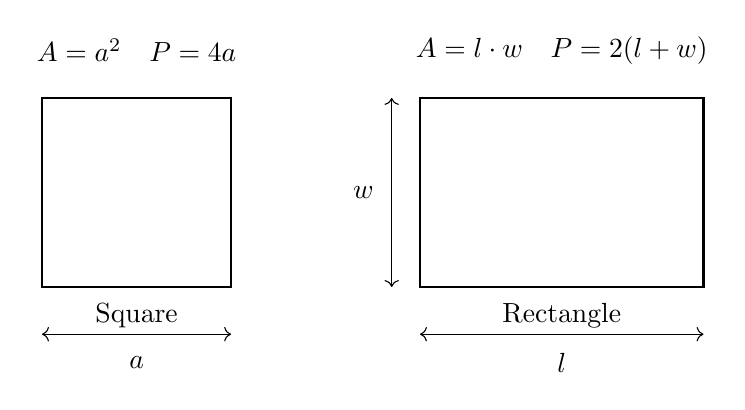
\begin{tikzpicture}[scale=1.2]
		% Square
		\draw[thick] (0,0) rectangle (2,2);
		\node at (1,-0.3) {Square};
		\draw[<->] (0,-0.5) -- (2,-0.5);
		\node at (1,-0.8) {\(a\)};
		\node at (1,2.5) {\(A = a^2 \quad P = 4a\)};

		% Rectangle
		\draw[thick] (4,0) rectangle (7,2);
		\node at (5.5,-0.3) {Rectangle};
		\draw[<->] (4,-0.5) -- (7,-0.5);
		\node at (5.5,-0.8) {\(l\)};
		\draw[<->] (3.7,0) -- (3.7,2);
		\node at (3.4,1) {\(w\)};
		\node at (5.5,2.5) {\(A = l \cdot w \quad P = 2(l+w)\)};
	\end{tikzpicture}
\end{center}

\subsection*{Circle and Triangle Types}
\begin{center}
	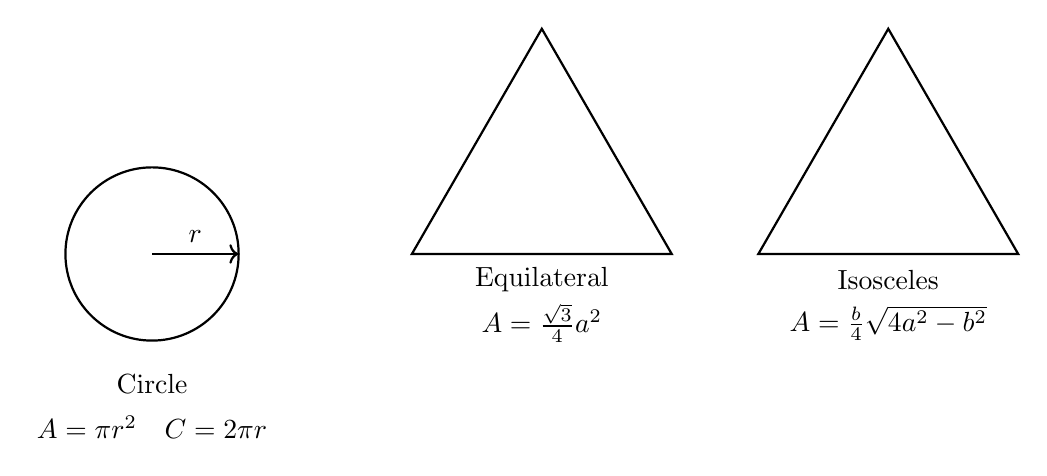
\begin{tikzpicture}[scale=1.1]
		% Circle
		\draw[thick] (0,0) circle(1cm);
		\draw[thick, ->] (0,0) -- (1,0);
		\node at (0.5,0.2) {\(r\)};
		\node at (0,-1.5) {Circle};
		\node at (0,-2) {\(A = \pi r^2 \quad C = 2\pi r\)};

		% Equilateral Triangle
		\draw[thick] (3,0) -- (4.5,2.6) -- (6,0) -- cycle;
		\node at (4.5,-0.3) {Equilateral};
		\node at (4.5,-0.8) {\(A = \frac{\sqrt{3}}{4} a^2\)};

		% Isosceles Triangle
		\draw[thick] (7,0) -- (8.5,2.6) -- (10,0) -- cycle;
		\node at (8.5,-0.3) {Isosceles};
		\node at (8.5,-0.8) {\(A = \frac{b}{4} \sqrt{4a^2 - b^2}\)};
	\end{tikzpicture}
\end{center}

\subsection*{Scalene Triangle, Trapezoid, Parallelogram}
\begin{center}
	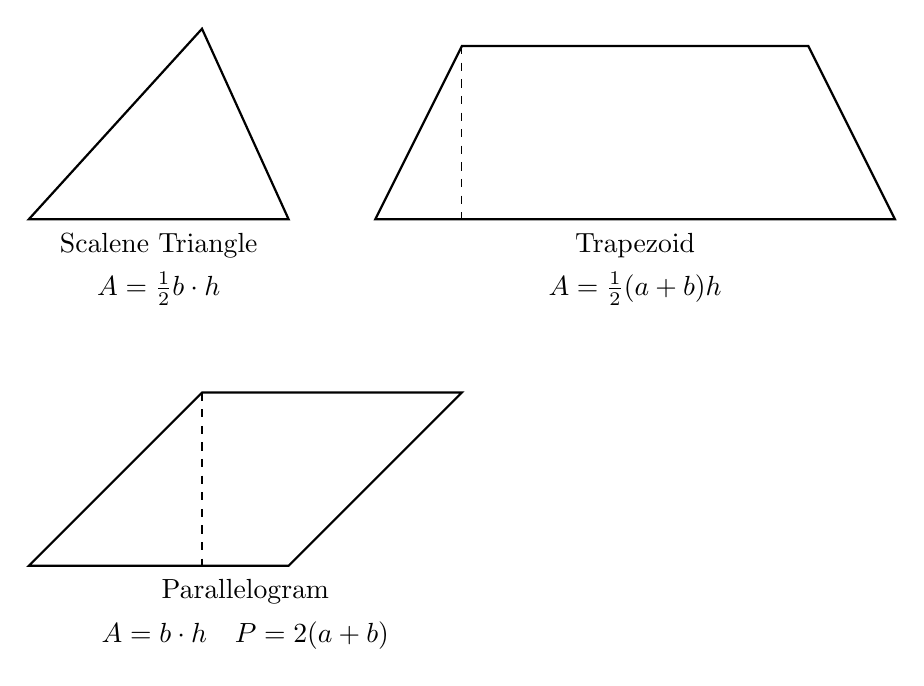
\begin{tikzpicture}[scale=1.1]
		% Scalene Triangle
		\draw[thick] (0,0) -- (2,2.2) -- (3,0) -- cycle;
		\node at (1.5,-0.3) {Scalene Triangle};
		\node at (1.5,-0.8) {\(A = \frac{1}{2} b \cdot h\)};

		% Trapezoid
		\draw[thick] (4,0) -- (5,2) -- (9,2) -- (10,0) -- cycle;
		\draw[dashed] (5,2) -- (5,0);
		\node at (7,-0.3) {Trapezoid};
		\node at (7,-0.8) {\(A = \frac{1}{2}(a+b)h\)};

		% Parallelogram
		\draw[thick] (0,-4) -- (2,-2) -- (5,-2) -- (3,-4) -- cycle;
		\draw[dashed] (2,-2) -- (2,-4);
		\node at (2.5,-4.3) {Parallelogram};
		\node at (2.5,-4.8) {\(A = b \cdot h \quad P = 2(a + b)\)};
	\end{tikzpicture}
\end{center}

\subsection{3D Geometric Figures with Formulas}

\subsubsection{Cube and Cylinder}
\begin{center}
	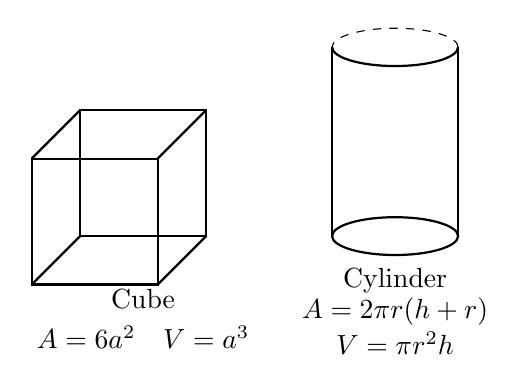
\begin{tikzpicture}[scale=0.8]
		% Cube
		\draw[thick] (0,0,0) -- (2,0,0) -- (2,2,0) -- (0,2,0) -- cycle;
		\draw[thick] (0,0,0) -- (0,0,2);
		\draw[thick] (2,0,0) -- (2,0,2);
		\draw[thick] (2,2,0) -- (2,2,2);
		\draw[thick] (0,2,0) -- (0,2,2);
		\draw[thick] (0,0,2) -- (2,0,2) -- (2,2,2) -- (0,2,2) -- cycle;
		\node at (1,-1) {Cube};
		\node at (1,-1.6) {\(A = 6a^2 \quad V = a^3\)};

		% Cylinder
		\begin{scope}[xshift=5cm]
			\draw[thick] (0,0) ellipse (1 and 0.3);
			\draw[thick] (-1,0) -- (-1,3);
			\draw[thick] (1,0) -- (1,3);
			\draw[thick] (-1,3) arc (180:360:1 and 0.3);
			\draw[dashed] (1,3) arc (0:180:1 and 0.3);
			\node at (0, -0.7) {Cylinder};
			\node at (0, -1.2) {\(A = 2\pi r(h + r)\)};
			\node at (0, -1.7) {\(V = \pi r^2 h\)};
		\end{scope}
	\end{tikzpicture}
\end{center}

\subsubsection{Cone and Sphere}
\begin{center}
	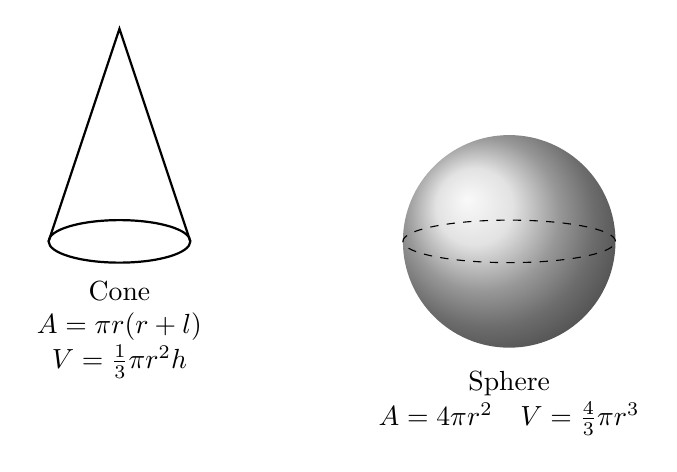
\begin{tikzpicture}[scale=0.9]
		% Cone
		\draw[thick] (0,0) ellipse (1 and 0.3);
		\draw[thick] (-1,0) -- (0,3) -- (1,0);
		\draw[dashed] (1,0) arc (0:180:1 and 0.3);
		\node at (0,-0.7) {Cone};
		\node at (0,-1.2) {\(A = \pi r(r + l)\)};
		\node at (0,-1.7) {\(V = \frac{1}{3} \pi r^2 h\)};

		% Sphere
		\begin{scope}[xshift=5.5cm]
			\shade[ball color=gray!30] (0,0) circle (1.5);
			\draw[dashed] (0,0) ellipse (1.5 and 0.3);
			\node at (0,-2) {Sphere};
			\node at (0,-2.5) {\(A = 4\pi r^2 \quad V = \frac{4}{3} \pi r^3\)};
		\end{scope}
	\end{tikzpicture}
\end{center}

\subsubsection{Pyramid and Prism}
\begin{center}
	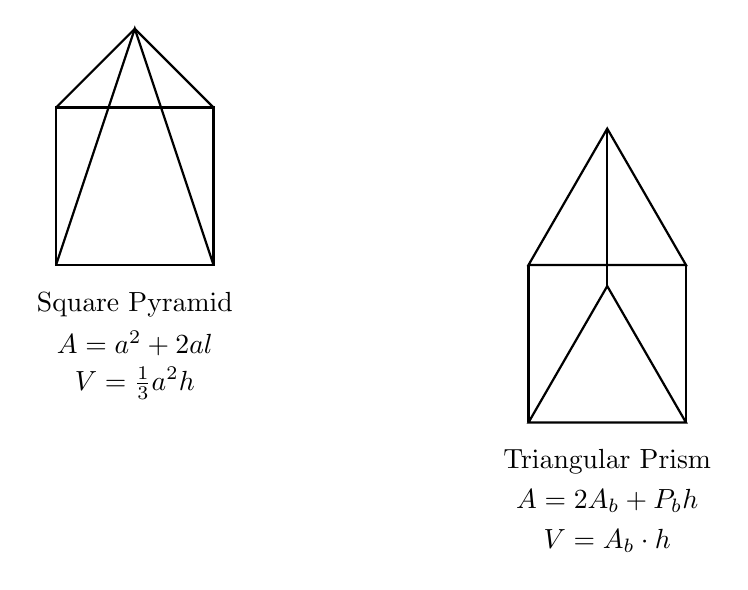
\begin{tikzpicture}[scale=1]
		% Square Pyramid
		\draw[thick] (0,0) -- (2,0) -- (2,2) -- (0,2) -- cycle;
		\draw[thick] (0,0) -- (1,3) -- (2,0);
		\draw[thick] (2,2) -- (1,3) -- (0,2);
		\node at (1,-0.5) {Square Pyramid};
		\node at (1,-1) {\(A = a^2 + 2al\)};
		\node at (1,-1.5) {\(V = \frac{1}{3}a^2 h\)};

		% Triangular Prism
		\begin{scope}[xshift=6cm]
			\draw[thick] (0,0) -- (2,0) -- (1,1.732) -- cycle;
			\draw[thick] (0,0) -- (0,-2);
			\draw[thick] (2,0) -- (2,-2);
			\draw[thick] (1,1.732) -- (1,-0.268);
			\draw[thick] (0,-2) -- (2,-2) -- (1,-0.268) -- cycle;
			\node at (1,-2.5) {Triangular Prism};
			\node at (1,-3) {\(A = 2A_b + P_b h\)};
			\node at (1,-3.5) {\(V = A_b \cdot h\)};
		\end{scope}
	\end{tikzpicture}
\end{center}

\subsection{Axioms of Euclidean Geometry}

Euclidean geometry is founded on a set of basic assumptions known as axioms or postulates, originally formulated by the Greek mathematician Euclid in his work \textit{Elements}. These axioms form the logical basis for plane geometry and include the following:

\begin{enumerate}
    \item \textbf{Axiom 1 (Line Postulate):} A straight line segment can be drawn joining any two points.
    
    \item \textbf{Axiom 2 (Extension Postulate):} Any straight line segment can be extended indefinitely in a straight line.
    
    \item \textbf{Axiom 3 (Circle Postulate):} Given any straight line segment, a circle can be drawn having the segment as radius and one endpoint as center.
    
    \item \textbf{Axiom 4 (Right Angle Postulate):} All right angles are congruent.
    
    \item \textbf{Axiom 5 (Parallel Postulate):} If a line segment intersects two straight lines and makes the interior angles on the same side less than two right angles, then the two lines, if extended indefinitely, meet on that side.
\end{enumerate}

These five postulates define the framework of classical geometry in a flat (Euclidean) space. Notably, the fifth postulate—the parallel postulate—has been the subject of much scrutiny and led to the development of non-Euclidean geometries when it was altered or replaced.

\subsection{Types of Angles and Angle Relationships}





\section{Constructing Triangles from Angles and Sides}
A triangle can be uniquely determined (up to congruence) using different combinations of sides and angles. The main construction cases are as follows:

\subsection{SSS (Side-Side-Side)}
A triangle is uniquely determined if all three sides are known.
\begin{center}
\begin{tikzpicture}[scale=1]
\draw[thick] (0,0) -- (5,0) node[midway, below] {$c$};
\draw[thick] (0,0) -- (2,3.5) node[midway, left] {$b$};
\draw[thick] (5,0) -- (2,3.5) node[midway, right] {$a$};
\node[below left] at (0,0) {$A$};
\node[below right] at (5,0) {$B$};
\node[above] at (2,3.5) {$C$};
\end{tikzpicture}
\end{center}

\subsection{SAS (Side-Angle-Side)}
A triangle is uniquely determined if two sides and the included angle are known.
\begin{center}
\begin{tikzpicture}[scale=1]
\coordinate (A) at (0,0);
\coordinate (B) at (5,0);
\coordinate (C) at (1.8,3);
\draw[thick] (A) -- (B) node[midway, below] {$c$};
\draw[thick] (A) -- (C) node[midway, left] {$b$};
\draw[thick] (B) -- (C) node[midway, right] {$a$};
\pic["$\theta$", draw=black, angle radius=1cm, angle eccentricity=1.3] {angle=B--A--C};
\node[below left] at (A) {$A$};
\node[below right] at (B) {$B$};
\node[above] at (C) {$C$};
\end{tikzpicture}
\end{center}

\subsection{ASA (Angle-Side-Angle)}
A triangle is uniquely determined if two angles and the included side are known.
\begin{center}
\begin{tikzpicture}[scale=1]
\coordinate (A) at (0,0);
\coordinate (B) at (5,0);
\coordinate (C) at (2,3.5);
\draw[thick] (A) -- (B) node[midway, below] {$c$};
\draw[thick] (A) -- (C);
\draw[thick] (B) -- (C);
\pic["$\alpha$", draw=black, angle radius=1cm, angle eccentricity=1.4] {angle=B--A--C};
\pic["$\beta$", draw=black, angle radius=1cm, angle eccentricity=1.4] {angle=C--B--A};
\node[below left] at (A) {$A$};
\node[below right] at (B) {$B$};
\node[above] at (C) {$C$};
\end{tikzpicture}
\end{center}

\subsection{AAS (Angle-Angle-Side)}
A triangle is uniquely determined if two angles and a non-included side are known.
\begin{center}
\begin{tikzpicture}[scale=1]
\coordinate (A) at (0,0);
\coordinate (C) at (4,0);
\coordinate (B) at (2,3);
\draw[thick] (A) -- (C) node[midway, below] {$b$};
\draw[thick] (A) -- (B);
\draw[thick] (B) -- (C);
\pic["$\alpha$", draw=black, angle radius=1cm, angle eccentricity=1.4] {angle=C--A--B};
\pic["$\beta$", draw=black, angle radius=1cm, angle eccentricity=1.4] {angle=A--C--B};
\node[below left] at (A) {$A$};
\node[below right] at (C) {$C$};
\node[above] at (B) {$B$};
\end{tikzpicture}
\end{center}

\subsection{SSA (Side-Side-Angle)}
Two sides and a non-included angle do \textbf{not always} determine a unique triangle. This case is ambiguous and can result in:
\begin{itemize}
    \item One triangle (when the opposite side is long enough),
    \item Two triangles (ambiguous case),
    \item No triangle (when the side is too short).
\end{itemize}
\begin{center}
\begin{tikzpicture}[scale=1]
\coordinate (A) at (0,0);
\coordinate (C) at (4,0);
\coordinate (B1) at (2,3); % triangle 1
\coordinate (B2) at (2,-2); % triangle 2
\draw[thick] (A) -- (C) node[midway, below] {$c$};
\draw[thick] (A) -- (B1) node[midway, left] {$b$};
\draw[thick] (A) -- (B2) node[midway, left] {$b$};
\draw[thick, dashed] (B2) -- (C);
\draw[thick] (B1) -- (C);
\pic["$\alpha$", draw=black, angle radius=1cm, angle eccentricity=1.4] {angle=C--A--B1};
\node[below left] at (A) {$A$};
\node[below right] at (C) {$C$};
\node[above] at (B1) {$B_1$};
\node[below] at (B2) {$B_2$};
\end{tikzpicture}
\end{center}

\subsection{Intercept Theorems}

The intercept theorems describe relationships between segment lengths when two rays from a point intersect two parallel lines. They are based on similar triangles and allow us to calculate unknown lengths using proportions.

\subsubsection{First Intercept Theorem}

If two rays start from a common point and are intersected by two parallel lines, then:

\[
	\frac{a}{a'} = \frac{b}{b'}
\]

\noindent where \(a\) and \(b\) are segments on one ray, and \(a'\), \(b'\) are the corresponding segments on the other ray.

\begin{center}
	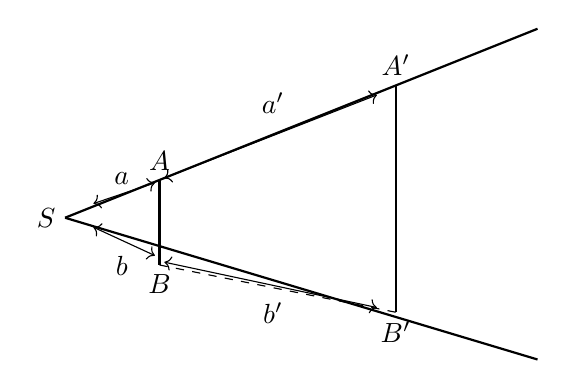
\begin{tikzpicture}[scale=1.2]
		% Rays
		\draw[thick] (0,0) -- (5,2); % upper ray
		\draw[thick] (0,0) -- (5,-1.5); % lower ray

		% Parallels
		\draw[thick] (1,0.4) -- (1,-0.5);
		\draw[thick] (3.5,1.4) -- (3.5,-1);

		% Points
		\node at (-0.2,0) {\(S\)};
		\node[above] at (1,0.4) {\(A\)};
		\node[below] at (1,-0.5) {\(B\)};
		\node[above] at (3.5,1.4) {\(A'\)};
		\node[below] at (3.5,-1) {\(B'\)};

		% Helper lines
		\draw[dashed] (1,0.4) -- (3.5,1.4);
		\draw[dashed] (1,-0.5) -- (3.5,-1);

		% Length labels
		\draw[<->] (0.3,0.15) -- (0.95,0.37);
		\node[above] at (0.6,0.25) {\(a\)};
		\draw[<->] (1.05,0.42) -- (3.3,1.3);
		\node[above] at (2.2,1) {\(a'\)};

		\draw[<->] (0.3,-0.1) -- (0.95,-0.4);
		\node[below] at (0.6,-0.3) {\(b\)};
		\draw[<->] (1.05,-0.47) -- (3.3,-0.95);
		\node[below] at (2.2,-0.8) {\(b'\)};
	\end{tikzpicture}
\end{center}

\subsubsection{Second Intercept Theorem (General Form)}

If a ray intersects two parallel lines, the segments from the origin point to the lines are in the same ratio as the segments along the parallels:

\[
	\frac{SA}{SA'} = \frac{SB}{SB'} \quad \text{and} \quad \frac{AB}{A'B'} = \frac{SA}{SA'}
\]

\begin{center}
	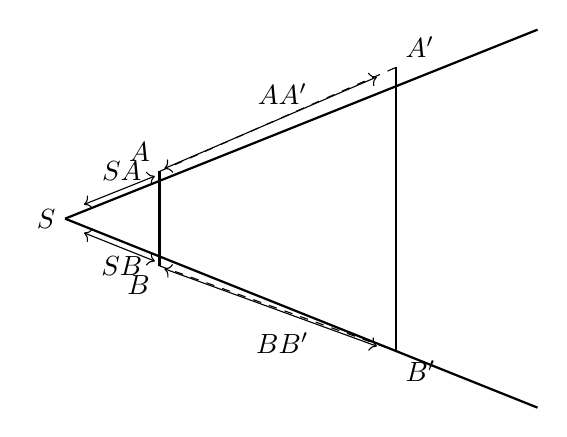
\begin{tikzpicture}[scale=1.2]
		% Rays
		\draw[thick] (0,0) -- (5,2); % upper ray
		\draw[thick] (0,0) -- (5,-2); % lower ray

		% Parallels
		\draw[thick] (1,0.5) -- (1,-0.5);
		\draw[thick] (3.5,1.6) -- (3.5,-1.4);

		% Points
		\node at (-0.2,0) {\(S\)};
		\node[above left] at (1,0.5) {\(A\)};
		\node[below left] at (1,-0.5) {\(B\)};
		\node[above right] at (3.5,1.6) {\(A'\)};
		\node[below right] at (3.5,-1.4) {\(B'\)};

		% Helper lines
		\draw[dashed] (1,0.5) -- (3.5,1.6);
		\draw[dashed] (1,-0.5) -- (3.5,-1.4);
		\draw[dashed] (1,0.5) -- (1,-0.5);
		\draw[dashed] (3.5,1.6) -- (3.5,-1.4);

		% Length labels
		\draw[<->] (0.2,0.15) -- (0.95,0.45);
		\node[above] at (0.6,0.3) {\(SA\)};
		\draw[<->] (1.05,0.53) -- (3.3,1.5);
		\node[above] at (2.3,1.1) {\(AA'\)};

		\draw[<->] (0.2,-0.15) -- (0.95,-0.45);
		\node[below] at (0.6,-0.3) {\(SB\)};
		\draw[<->] (1.05,-0.53) -- (3.3,-1.35);
		\node[below] at (2.3,-1.1) {\(BB'\)};
	\end{tikzpicture}
\end{center}

\newpage





\end{document}
